%% =====================================================================
%% Anschreiben — ALTEN GmbH · Software Architect (Refactoring) (all gender)
%% moderncv class (Fonts/Icons), aber EIGENER kompakter, einzeiliger Header
%% statt der mehrzeiligen moderncv-Briefkopf-Mechanik.
%% Language: DE (matched to the job posting). Compile with MiKTeX:
%%   pdflatex coverletter_alten_software-architect.tex
%% =====================================================================

\documentclass[10pt,a4paper]{moderncv}
\moderncvstyle{banking}     % (nur für Fonts/Setup; Header ist unten custom)
\moderncvcolor{blue}

% ---- Encoding & language -------------------------------------------
\usepackage[utf8]{inputenc}
\usepackage[T1]{fontenc}
\usepackage[ngerman]{babel}
\usepackage[scale=0.82]{geometry}

% ===== FONT-TEST: genau EINE der folgenden Zeilen aktiv lassen ======
% (die anderen mit % auskommentieren, dann neu kompilieren)
\usepackage{lmodern}                                              % Latin Modern (Standard, wie CV)
% \usepackage[sfdefault]{FiraSans}                                % Fira Sans (modern, technisch)
% \usepackage[default]{lato}\renewcommand{\familydefault}{\sfdefault}      % Lato (freundlich, rund)
% \usepackage{carlito}\renewcommand{\familydefault}{\sfdefault}   % Carlito (Calibri-ähnlich)
% \usepackage{XCharter}                                           % XCharter (moderne Serife)
% \usepackage[sfdefault]{noto}                                    % Noto Sans (neutral, klar)
% ====================================================================

% ---- Extra packages for note, table --------------------------------
\usepackage{tcolorbox}
\usepackage{graphicx}
\usepackage{tabularx}
\usepackage{booktabs}
\usepackage{array}
% NOTE: fontawesome6 wird bereits von moderncv geladen — NICHT erneut laden.

% ---- Colors --------------------------------------------------------
\definecolor{accent}{HTML}{2C6E91}
\definecolor{ink}{HTML}{222222}
\definecolor{light}{HTML}{777777}
\definecolor{strongc}{HTML}{1F8A57}
\definecolor{partialc}{HTML}{C98A1B}
\definecolor{adjac}{HTML}{8A8A8A}
\definecolor{notebg}{HTML}{EAF2F6}

% ---- Strength badges (fontawesome6 names) --------------------------
\newcommand{\badge}[2]{\textcolor{#1}{\footnotesize\textbf{#2}}}
\newcommand{\strong}{\badge{strongc}{\faCircle\ stark}}
\newcommand{\partialm}{\badge{partialc}{\faCircleHalfStroke\ teilw.}}
\newcommand{\adjacent}{\badge{adjac}{\faRegistered\ angrenz.}}

% Sender name (moderncv benötigt \name gesetzt; Header ist unten custom)
\name{Andreas}{Butry}

\begin{document}

% ---- Kompakter, einzeiliger Header ---------------------------------
{\Huge\bfseries\color{accent}Andreas Butry}\\[1pt]
{\small\color{light}Funktionale Sicherheit, Software Qualität, Engineering-Prozesse \& KI-Innovation}\\[5pt]
{\color{accent}\rule{\linewidth}{1pt}}\\[4pt]
{\small\color{ink}%
\faLocationDot~Louise-Schroeder-Str.\ 2, 67551 Worms, Germany \;\textcolor{accent}{|}\;
\faPhone~+49\,179\,140\,90\,57 \;\textcolor{accent}{|}\;
\faEnvelope~\href{mailto:andreas.butry@gmail.com}{andreas.butry@gmail.com}\\[3pt]
\faGlobe~\href{https://andreasbutry.github.io/mypage/}{andreasbutry.github.io/mypage} \;\textcolor{accent}{|}\;
\faLinkedin~\href{https://www.linkedin.com/in/andreas-butry-23641530a}{LinkedIn-Profil}}

\bigskip

% ---- Empfänger & Datum ---------------------------------------------
\begin{minipage}[t]{0.62\linewidth}
  ALTEN GmbH\\
  Personalabteilung / Recruiting
\end{minipage}\hfill
\begin{minipage}[t]{0.33\linewidth}
  \raggedleft Worms, \today
\end{minipage}

\bigskip

% ---- Betreff -------------------------------------------------------
{\bfseries Bewerbung als \emph{Software Architect (Refactoring) (all gender)}}

\medskip

% ---- Transparenzhinweis --------------------------------------------
\begin{tcolorbox}[colback=notebg,colframe=accent,boxrule=0.8pt,arc=3pt,
                  left=8pt,right=8pt,top=5pt,bottom=5pt]
{\small\color{ink}\faRobot\enspace\textbf{Transparenzhinweis.}
Dieses Anschreiben wurde \textbf{in Teilen von einer KI-Automatisierung
geschrieben, die ich selbst entwickelt habe}: Sie liest die
Stellenausschreibung, erkennt deren Sprache, gleicht die Anforderungen mit
meiner Erfahrung ab ($\rightarrow$ \emph{Eignungstabelle auf Seite~2}) und
verfasst Teile des Anschreibens in der Sprache der Ausschreibung. Wie ich arbeite, sehen Sie
also bereits an diesem Dokument.}
\end{tcolorbox}

\medskip

Sehr geehrte Damen und Herren,

\medskip

% ---- Body: values-first (lowercase first word after the comma) -----
gutes Refactoring bedeutet für mich, \textbf{Komplexität
herunterzubrechen}, \textbf{das große Ganze einer Codebase im Blick zu behalten}
und jede Änderung mit einem klaren \textbf{Verifikations-Mindset} (z.\,B. Test-Driven Development) abzusichern.
Diese Haltung habe ich in über acht Jahren sicherheitskritischer
Softwareentwicklung verinnerlicht, und genau sie möchte ich als
\emph{Software Architect} bei ALTEN einbringen.

In \textbf{C} habe ich über Jahre Embedded-Software auf Steuergeräten entwickelt
und optimiert, in \textbf{Python} automatisiere ich heute Entwicklungs- und
KI-Workflows. Software- und Systemarchitektur habe ich über den gesamten
Lebenszyklus verantwortet: von den Anforderungen über die Architektur bis zur
Verifikation und Freigabe nach definierten Entwicklungsprozessen (z.\,B.
ISO~26262 und ASPICE). Gewachsene, komplexe
Strukturen behutsam umzugestalten, gehörte dabei zu meinem Alltag.

Neben der Technik ist mir ein Punkt besonders wichtig: ein menschlicher,
respektvoller Umgang im Team, gerade dann, wenn es einmal schwierig wird. Gute
Architektur lebt für mich genauso von klarer Kommunikation und Vertrauen wie von
sauberem Code. Bei TES Electronics verantworte ich System- und
Softwareentwicklung für eingebettete Geräte, vernetzte Produkte und
Cloud-Services und baue zugleich Entwicklungsprozesse für KI-generierte Software
mit agentischen Workflows auf, etwa zur Automatisierung von Code-Reviews und
Refactorings (stets mit menschlichem Review-Anteil, Konzept
\hyperlink{hitl}{\textbf{Human-in-the-Loop}} $\rightarrow$ Seite~2). Wie gut Ihre Anforderungen zu meiner Erfahrung
passen, habe ich auf Seite~2 in einer \textbf{Eignungstabelle} zusammengestellt.

Über ein persönliches Gespräch, in dem wir herausfinden, ob wir zueinander
passen, würde ich mich sehr freuen.

% ---- Grußformel ----------------------------------------------------
\bigskip
Mit freundlichen Grüßen,\\[2.0em]
Andreas Butry

\medskip
{\small\color{light}Anlagen: Lebenslauf, Zeugnisse}

% ---- Werte-Liste (Seite 1) -----------------------------------------
\medskip
{\color{accent}\rule{\linewidth}{0.6pt}}\\[3pt]
{\small\bfseries\color{accent}Meine Engineering-Werte}\par\smallskip
{\small
\newcommand{\valitem}[3]{\par\noindent{\color{accent}#1}~\textbf{#2}: #3\par\vspace{1.5pt}}
\valitem{\faSitemap}{Komplexität herunterbrechen}{Strukturierte Arbeitspakete mit klaren Schnittstellen und Validierungspfaden.}
\valitem{\faDiagramProject}{Das große Ganze sehen}{Anforderungen, System, Prozesse und Stakeholder zusammen denken.}
\valitem{\faComments}{Klare Kommunikation}{Technische Themen verständlich machen und früh abstimmen.}
\valitem{\faCheckDouble}{Qualitätsfokus}{Traceability, Review-Disziplin und Verifikations-Mindset.}
\valitem{\faSeedling}{Kontinuierliches Lernen}{Methoden und Workflows verbessern, an Fehlern wachsen.}
\valitem{\faHandsHolding}{Menschlich \& empathisch}{Ruhig, respektvoll und lösungsorientiert.}
\valitem{\faShare}{Wissen teilen}{Dokumentation, Mentoring und offener Austausch.}
}

% =====================================================================
% APPENDIX (Seite 2): Eignungstabelle
% =====================================================================
\clearpage

{\Large\bfseries\color{accent}Eignungstabelle — Anforderungen \& Erfahrung}\\[2pt]
{\small\color{light}Automatisch aus der Ausschreibung abgeleitet und mit meinem
Profil abgeglichen. Legende:\;\strong\;\;\partialm\;\;\adjacent}

\medskip

\renewcommand{\arraystretch}{1.45}
\setlength{\tabcolsep}{10pt}
\begin{tabularx}{\linewidth}{@{}>{\raggedright\arraybackslash}p{0.28\linewidth} @{\hspace{16pt}} >{\raggedright\arraybackslash}X @{\hspace{16pt}} >{\centering\arraybackslash}p{0.13\linewidth}@{}}
\toprule
\textbf{Anforderung (Ausschreibung)} & \textbf{Beleg aus meiner Erfahrung} & \textbf{Match}\\
\midrule
Programmierung in C und Python & C in Echtzeit-/Embedded-Systemen (Steuergeräte, HIL); Python für Automatisierung, Tooling \& KI-Workflows & \strong\\
Codebase optimieren / Refactoring & Aufbau \& Optimierung von Entwicklungsprozessen; KI-gestützte Code-Reviews; Qualität via MISRA-C, Polyspace \& HIS-Metriken & \strong\\
Komplexe Strukturen umgestalten & „Komplexität herunterbrechen``: Umstrukturierung komplexer Regelungs-Algorithmen \& Architekturen & \strong\\
Software- \& Systemarchitektur & System-/SW-Architektur von Anforderungen bis Validierung; redundante Zwei-ECU-Architektur & \strong\\
Linux und Baremetal & Embedded-Entwicklung auf Steuergeräten (Baremetal/RTOS); Linux im Entwicklungs-Stack & \partialm\\
Studium (SE, Control Systems, Comp.\ Eng., Mathe, Physik o.\,ä.) & M.Sc.\ Elektro- \& Informationstechnik, TU Darmstadt & \strong\\
Berufserfahrung SW-Entwicklung \& Architektur & 8+ Jahre @ Continental (sicherheitskritisch) und TES Electronics & \strong\\
Englisch verhandlungssicher, idealerw.\ Deutsch & Deutsch Muttersprache; Englisch verhandlungssicher & \strong\\
\bottomrule
\end{tabularx}

% ---- Human-in-the-Loop-Grafik (unter der Tabelle) ------------------
\bigskip
\hypertarget{hitl}{}
{\Large\bfseries\color{accent}Konzept: Human-in-the-Loop}\\[2pt]
{\small\color{light}Aufbau meiner agentischen Workflows bei TES: jeder KI-Agent
mit menschlicher Prüfung und Freigabe vor dem nächsten Schritt.}

\smallskip

\begin{center}
  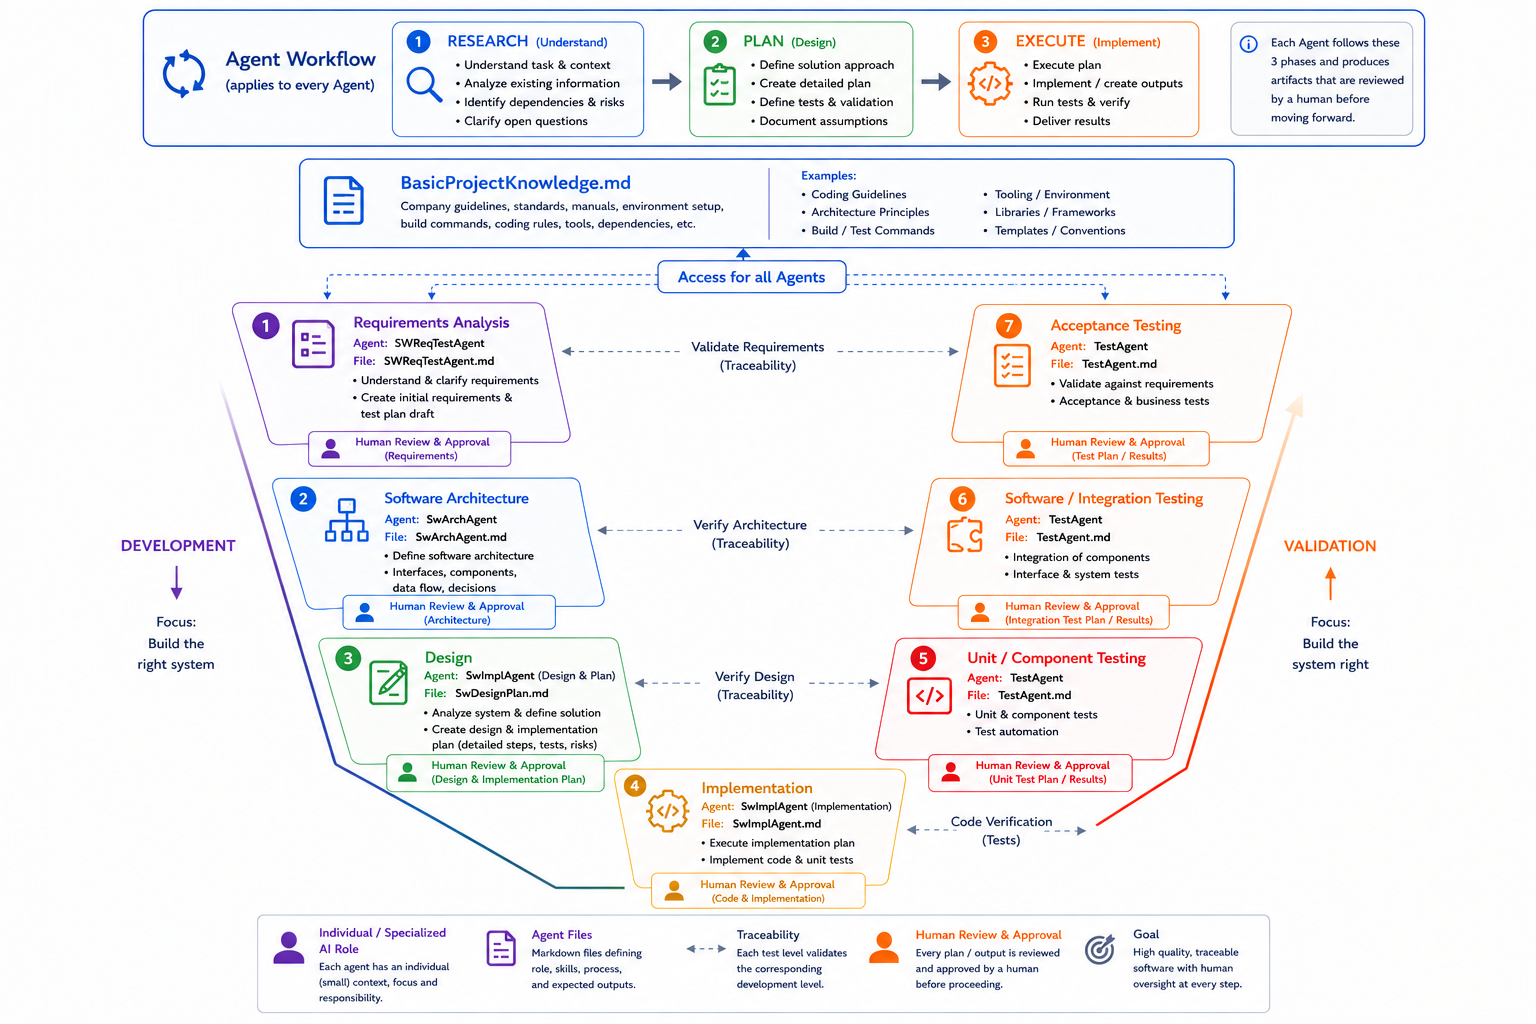
\includegraphics[width=0.9\linewidth]{../../agents_in_sldc_final.png}
\end{center}

\end{document}
